% Created 2022-03-16 Wed 00:51
% Intended LaTeX compiler: pdflatex
\documentclass[11pt]{article}
\usepackage[utf8]{inputenc}
\usepackage[T1]{fontenc}
\usepackage{graphicx}
\usepackage{longtable}
\usepackage{wrapfig}
\usepackage{rotating}
\usepackage[normalem]{ulem}
\usepackage{amsmath}
\usepackage{amssymb}
\usepackage{capt-of}
\usepackage{hyperref}
\usepackage{gensymb}
\usepackage{circuitikz}
\usepackage{tikz}
\usepackage{minted}
\usepackage[margin=2cm]{geometry}
\usepackage{url}
\usepackage{tikz}
\usepackage{float}
\usepackage{gensymb}
\usepackage{amsmath}
\numberwithin{equation}{section}
\usepackage{chngcntr}
\counterwithin{figure}{section}
\counterwithin{table}{section}
\usepackage{amssymb}
\newcommand {\R}{\mathbb{R}}
\usepackage{gensymb}
\usepackage{booktabs}
\usepackage{minted}[linenos]
\usepackage{sourcecodepro}
\definecolor{deepblue}{rgb}{0.0, 0.18, 0.39}
\setlength{\parindent}{0}
\usepackage{parskip}
\usepackage{enumitem}
\setlist{noitemsep}
\usepackage[format=plain, labelfont={bf}, textfont=it]{caption}
\usepackage{booktabs}
\usepackage[framemethod=tikz]{mdframed}
\BeforeBeginEnvironment{minted}{\begin{mdframed}[style=sourcecode]}
\AfterEndEnvironment{minted}{\end{mdframed}}
\author{Ben Frazer\thanks{2704250F@student.gla.ac.uk}}
\date{\today}
\title{The Need for Demand side Fast Frequency Response and Inertia in a Zero Carbon Grid}
\hypersetup{
 pdfauthor={Ben Frazer},
 pdftitle={The Need for Demand side Fast Frequency Response and Inertia in a Zero Carbon Grid},
 pdfkeywords={},
 pdfsubject={},
 pdfcreator={Emacs 27.2 (Org mode 9.6)}, 
 pdflang={English}}
\begin{document}

\maketitle
\tableofcontents

\mdfdefinestyle{sourcecode}{%
%backgroundcolor=darkgray,
skipabove=12pt,
hidealllines=true,
apptotikzsetting={%
  \tikzset{mdfbackground/.append style={fill=deepblue,fill opacity=0.1}}},
leftline=true,%innerleftmargin=10,innerrightmargin=10,
innerleftmargin=25,
linewidth = 4pt,
roundcorner = 2pt,
linecolor= darkgray,
%#frametitlerule=true,frametitlerulecolor=green,
%#frametitlebackgroundcolor=darkgray,
%#frametitlerulewidth=2pt
}
\section{Introduction}
\label{sec:orga6a7785}
The UK government has committed to the target of becoming net zero by 2050. This commitment is just one of the many similar such commitments to net zero made by governments all around the world. In this essay I will explore how a truly zero carbon grid could be realised with current technology, and with this framework highlight the fundamental trade-off and constrains which must be reconciled as a part of this transition.
\section{Zero carbon Energy Mix}
\label{sec:org3cb08e6}
Forecasting the future energy mix is the subject of extensive debate and is sensitive to a huge variety of unpredictable factors and unknowns such as government policy, geopolitical developments, to disruptive technologies. This analysis however starts with the assumption that the UK grid is indeed to be truly decarbonized and attempts to reason how this might look with current technologies. In this section will investigate which combination of technologies would likely provide the bulk of energy. The technologies considered here will simply be based on the current dominant sources of renewable and zero carbon energy on the UK grid shown in Figure \ref{figPie2020CumGen} as the only other dominant zero carbon energy source.

\begin{figure}[H]
\centering
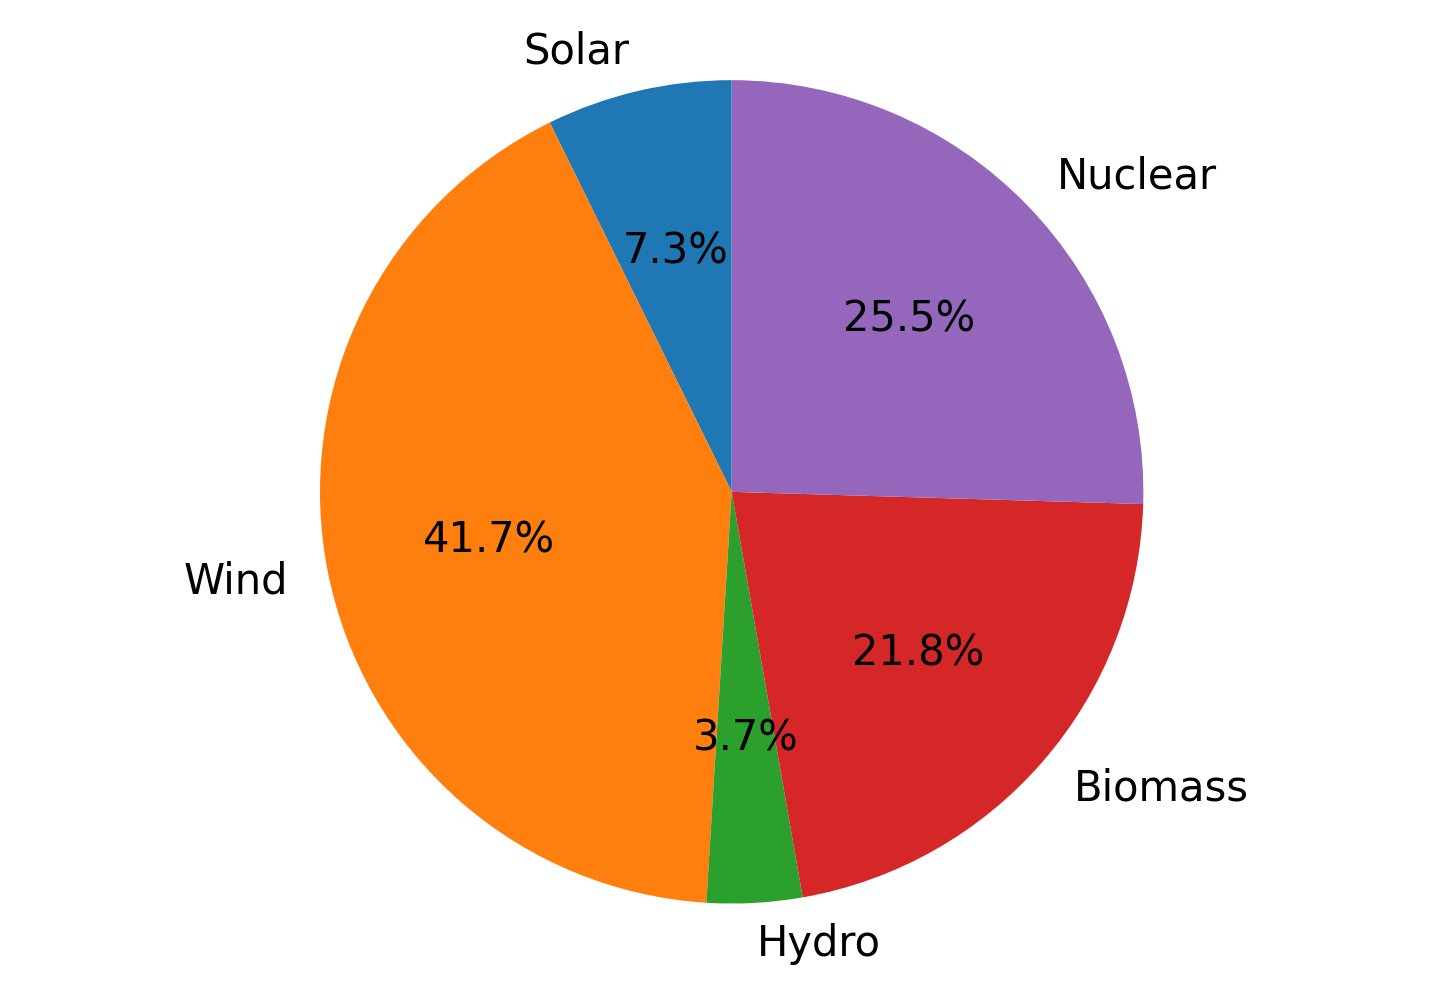
\includegraphics[width=0.8\textwidth]{./.ob-jupyter/9d5f54f66e0860cfcadd03202a7835f8eee375c2.png}
\caption{\label{figPie2020CumGen}Breakdown of UK zero carbon energy production (Wave/tidal Excluded due to low scale) in GWh for the year 2020-2021 based on UK government data \cite{RenewableElecricityCap}}
\end{figure}

\subsection{Solar}
\label{sec:orgaeda9e6}
\subsection{Offshore Wind}
\label{sec:orga7acf60}
\subsection{Nuclear}
\label{sec:orgbd698d4}
Nuclear energy has amongst the highest levelized
Given the
\subsection{Biomass \label{secBioGas}}
\label{sec:orgc15d623}
This section will be concerned with exploring the scalability and potential role that biomass may play in the future energy mix. For clarity, ``biomass'' in this essay will refer to a subset of generation types which produce energy from once living organisms \footnote{Note recently living i.e. not fossils} either by direct combustion or by generating gas through anerobic digestion.

A breakdown of the various technologies that constitute biomass energy is shown in Figure \ref{figPie2020BiomassBreakdown}. The reader should note that the totality of this chart represents only roughly 12.6\% of the total UK electrical energy production that energy in the year 2020 \cite{BiomassPolicyStatement}. Many of these technologies vary substantially in their scalability and as such the following key technologies will be treated individually.

\begin{itemize}
\item Plant Biomass
\item Anaerobic Digestion
\item Energy from waste
\item Landfill Gas
\end{itemize}

Other biomass technology will not be considered in this report due to it's expected low future utilization.

\begin{figure}[H]
\centering
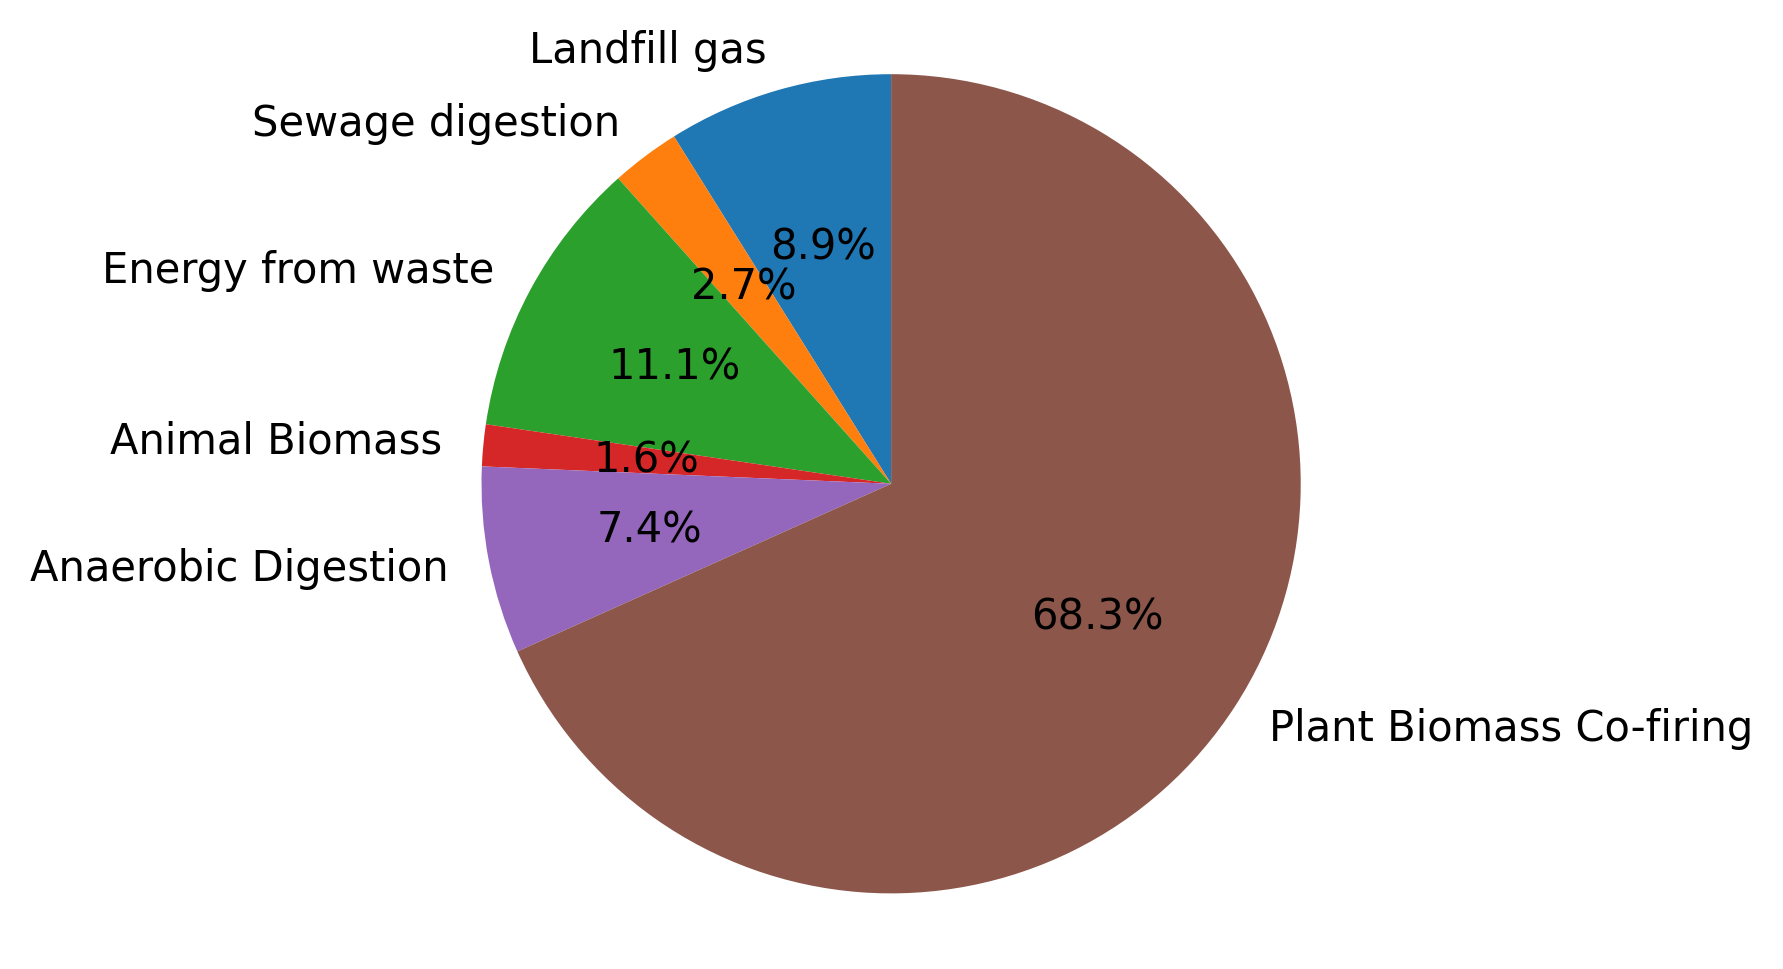
\includegraphics[width=0.8\textwidth]{./.ob-jupyter/603c0a61cc39a759145c8c2636878e943182f773.png}
\caption{\label{figPie2020BiomassBreakdown}Breakdown of ``biomass'' energy by type based on UK government data \cite{RenewableElecricityCap}[fn::For tabular data see Section \ref{secAppBiomassWasteEner}]}
\end{figure}

\subsubsection{Plant Biomass co-firing}
\label{sec:org03189aa}
Biomass co-firing involves the process of combusting certain types of feed-stock directly along side fossil fuels (usually coal) and is by far the dominant form of Biomass generation accounting for \(\approx\)68.3\% of total Biomass energy in the year 2020. The vast majority of this is in the form of wood bi-products and pellets imported from the united states and Canada \cite{BiomassPolicyStatement}.

Using such bio-fuels is net carbon neutral since the trees will regrow and recapture the emitted carbon, however there are still major concerns relating to the scalability of this technology.

One immediate concern on the suitability of co-firing for a zero carbon grid, is that it depends upon fossil fuels also being combusted. It is clearly possible to combust Biomass without using fossil fuels, but one of the key advantages of co-firing is that the combustion efficiency of the biomass is substantially improved due to the large scale and temperature of coal boilers. Further more there is a substantial increase in fouling and slagging when the percentage of biomass exceeds 50\% which also acts to decrease efficiency \cite{biomassNA}. Further more the costs of these bio fuels can be shown to be substantially higher than just coal which will be exacerbated with the decreased combustion efficiency incurred by high ratios of bio-fuel relative to coal. With many carbon capture schemes working in excess of 90\% efficiency, it is certainly possible that this may be mitigated in part or whole, however such schemes tend also to incur substantial increases in LCOE.

Currently the UK based co-firing schemes are heavily reliant on foreign imported feedstock in the form of wood pellets. Not only does the shipping of these pellets incur carbon emissions, it also hints at another inherent limit of this technology, that being land surface area. With the large majority of the UK being farmland, only around 13\% remains as forest, amounting to around 3.23 million hectares. The UK as a result is already heavily dependant on foreign timber for the building sector, though wooden pellets imports for co-firing are currently still the dominant import at 9.1MT.

With the current generation demand for feedstock well outpacing domestic production with even this limited scale of operations currently providing only \(\approx\)8.6\% of the current UK demand, it seems unlikely that this technology will scale substantially to replace coal or natural gas. It does however provide the interesting possibility of acting as a form of long term energy storage which may be dispatched to compensate from variable renewable sources.


\subsubsection{Scalability}
\label{sec:org51cf572}

\subsubsection{Plant Biomass LCOE}
\label{sec:orgb54dce0}

\subsection{Interconnects}
\label{sec:org76ba9fb}
\subsection{Impact}
\label{sec:org4d47a4a}
It is clear that a grid so heavily dependant on intermittent generation such as wind and solar, the available energy will fluctuate drastically both on a seasonal basis and on a relatively instantaneous basis. Though Offshore wind
\section{Constraints}
\label{sec:org4132870}
To bound the problem we may set constraints on aspects of this proposed future grid to help narrow down the problem.

\subsection{Cost of electricity}
\label{sec:org7b7fdc2}
Since we have established
\subsubsection{What is LCOE}
\label{sec:orgbc8f357}
Levelized cost of electricity (LCOE) is defined simply as the total cost of building, running and decommissioning an energy generation asset divided by it's lifetime generation cost.
\begin{align}
\label{eqLCOE}
LCOE = \frac{\text{Lifetime Cost (\$)}}{\text{Lifetime Production (KWh)}}
\end{align}

This is a vital metric for comparing the cost effectiveness and profitability of a given generation source. By accounting for profit margins and transmission/distribution use of system fees, this metric may also give a very rough insight into the likely end cost of energy to the consumer assuming a relatively competitive energy market.

\subsubsection{Breakdown of an energy Bill}
\label{sec:org8c06fae}
A vital constrain when considering future energy mix is that the cost of electricity to the end user remain low enough so that consumers will have manageable heating bills. This means that on a \$/kWh\footnote{\$/kWh is used for compatibility with the academic literature} heat energy must cost less than or in the region of the existing cost of gas. From this and the typical COP of a consumer grade heat pump, an upper limit on the acceptable cost per kWh may be established. This can then be roughly translated in an upper limit on the total LCOE of the generation sources on the network. From Figure \ref{figPieBillBreakdown}, we can see that the wholesale price of electricity, accounts for only \(\approx\)30\% of the final bill.

\begin{figure}[H]
\centering
\includegraphics[width=0.8\textwidth]{./.ob-jupyter/95852af655160b405263c78f83e0c6e2de1d2abc.png}
\caption{\label{figPieBillBreakdown}Ofgem Estimated components of customer's energy bills from Ofgem \cite{ofgemBillBreakdown}}
\end{figure}




\subsection{Consistency, Overcapacity and Energy Storage Trade-off}
\label{sec:org411f08f}
When faced with a highly variable energy supply one obvious degree of freedom is to oversize the system capacity. Though the minimum and maximum available generation would likely still vary with the same shape, the absolute value of the minimum would have increased meaning the absolute size of any generation shortfall, would be diminished. This has the obvious downside of resulting in a direct increase in costs due to the increased number/capacity of assets which would be directly be passed onto the levelized cost of electricity and thus the cost to the consumer. Where \emph{reliability} is defined as the fraction of time that demand is less than the available energy, one would expect there would be diminishing returns on \emph{reliability} for increases in capacity simply due to the statistical nature of renewable availability.

To fully derive the degree of capacity required to guarantee 100\% energy fundamentally depends on the statistical variation of the available energy of the renewable resources and the total energy storage capacity on the network. Producing an accurate figure for this is near to impossible would require complex statistical modelling along with substantial knowledge assumptions regarding the energy storage capacity of the network, thus the calculation conducted here should merely be seen as proving a ballpark figure.

Through a comprehensive study of observed wind speed data from 66 sites across the UK and statistical analysis, Sinden \cite{2007} showed that that the seasonal average wind power availability varies by only approximately \textpm{} 10\% of the yearly average. It was also shown that the total period of time per year where the entirety of the year where 90\% of the UK experiences low wind is less than one hour.

For this analysis, Wind and solar data from the UK website gridwatch \cite{gridwatch} for the year 2020-2021. By assuming that the entirety of the UK's wind resource is not curtailed due to \footnote{this may seem like a substantial assumption, but}


meaning  it would likely be require oversize Since a fundamental requirement of any stable grid be that reliability always be 100\% (i.e. available generation > demand)

It is therefore expected that for the lower cost generation sources such as solar and offshore wind, there will be substantial over capacity while the nuclear fission plants operate continuously at near full capacity.

\section{Future Energy Demand}
\label{sec:org43e10b6}
In this section I will briefly cover the likely trends in the UK's energy demand and what influence this may have on the electrical market. The three key areas of focus are:
\begin{itemize}
\item Heating Demand \ref{secHeating}
\item Data Centres \ref{secDataCenters}
\item Electric Vehicles \ref{secEVs}
\end{itemize}

\subsubsection{Heating \label{secHeating}}
\label{sec:orga9fb1d8}
A critical challenges in the transition to net zero is decarbonising residential space heating. As of \textit{<2022-03-15 Tue>}, the future of heating in the UK is still very unclear. Until recently the UK has relied on the abundant gas reserves of the north sea for the vast majority of it's heating needs. These reserves however are dwindling, and beyond being in carbon intensive, depending in imported natural gas is expected to incur increasing cost, not to mention poses a geopolitical vulnerability. It is thus no surprise that decarbonising heating has received substantial attention from the government.

The current policy of the UK government seems to be leaning in the direction of full electrification of heating using heat pumps in combination with altered building standards for improved insulation. This approach has been met with some scepticism on the grounds of high unit cost of heat-pumps and relatively limited uptake [ \texttt{citation needed} ]. It is the authors opinion however that these limitations may be mitigated though shared ownership of units or some form of district heating schemes.

Competing proposals have also been made to utilise the existing gas infrastructure instead with hydrogen generated through electrolyse rather than fossil fuel sourced gas \footnote{Biogas may also be used, however it seems unlikely that biogas will ever become a dominant source of heating due to fundamental limitations in available bio-matter}. This approach has the advantage of the relatively high energy density of hydrogen \footnote{This is relative to the current energy density of Lithium Ion battery} potentially allowing for relatively low cost energy storage [ \texttt{citation needed} ]. The potential advantages of hydrogen have also attracted significant attention in the transport sector, seeing research in cars, busses, trains and even boats. When competing with electrical storage such as batteries, or pumped hydro, it is still very unclear which, if any technology will decisively win-out in these sectors. If this were to occur,  it would likely substantial improve the economics of hydrogen for heating due to the potential to share infrastructure and in the benefits of research and commercial interest.

As such only two plausible futures exist for heating energy\footnote{It is noted that at least transiently, the end result will likely be some combination of both}:

\begin{enumerate}
\item Large scale Hydrogen gas network
\item Full Electrification using Heat-pumps
\end{enumerate}

When considered from the point of view of the electrical energy network, these two options are both fundamentally consumers of energy, however the quantity and distribution of the load vary substantially. First of all, green hydrogen must first be generated using electrolyse. Current alkaline fuel cell technology such as Cummin's HYDRLYZER can attain up to 70\% efficiency \cite{CuminsElectrolizer}. Depending on the application, the hydrogen may then need to be compressed for storage/transport. This stage can lead to a further energy cost which will vary depending on technology. It is possible that if suitable storage infrastructure existed hydrogen could be generated relatively independently of the instantaneous energy demand.
\subsubsection{Data Centres \label{secDataCenters}}
\label{sec:orgf69ac02}

\subsubsection{Electric Vehicles \label{secEVs}}
\label{sec:org68b57b0}

\section{Storage}
\label{sec:org1a98f66}
\subsection{Hydrogen CCGT}
\label{sec:orgb8cd4c6}
\subsection{Battery}
\label{sec:orgb5d79a8}
\subsection{Hydrogen Gas heating}
\label{sec:org96d1743}
\section{Frequency Control Mechanisms}
\label{sec:org3164676}
\subsection{Current}
\label{sec:orgdfda133}
\subsection{Future}
\label{sec:org37dbed3}
\subsubsection{VSM}
\label{sec:org938f2a9}
\subsubsection{Synchronous Condensers}
\label{sec:orgeec48dc}

\section{Appendices}
\label{sec:org17dcebe}
\subsection{Breakdown of a consumer energy bill}
\label{sec:org157e9f4}

\begin{table}[H]
\caption{\label{tabBillBreakdown}Ofgem Estimated components of customer's energy bills from Ofgem \cite{ofgemBillBreakdown}}
\centering
\begin{tabular}{rrrrrr}
VAT & Other Costs & Wholesale Price & Network Costs & Environmental/social obligation & Operating Costs\\
\hline
4.76 & 2.09 & 29.28 & 23.37 & 25.48 & 16.34\\
\end{tabular}
\end{table}

\subsection{Energy Mix}
\label{sec:org42d2268}
\begin{table}[H]
\caption{\label{tabUkGreenEnergy2020}Breakdown of UK renewable energy production in GWh for the year 2020-2021 based on UK government data \cite{RenewableElecricityCap}}
\centering
\begin{tabular}{lrrrrrrr}
 & Solar PV & Wind & Hydro & Biomass & Nuclear & wave / tidal & total\\
\hline
GWh & 13157.99 & 75369.14 & 6753.92 & 39311 & 46000 & 11.28 & 134592.05\\
Percent & 9.8 & 56.0 & 5.0 & 29.2 & 34.2 & 0.0 & \\
\end{tabular}
\end{table}

\subsection{Biomass/Waste Energy Breakdown \label{secAppBiomassWasteEner}}
\label{sec:orgef3118b}
\begin{table}[H]
\caption{\label{tabBiomassBreakdown}Breakdown of Energy generated from Biomass/Waste (GWh) according to UK government data \cite{RenewableElecricityCap}}
\centering
\begin{tabular}{lrrrrrrr}
\toprule
 & Landfill gas & Sewage digestion & Energy from waste & Animal Biomass & Anaerobic Digestion & Plant Biomass & Total\\
\midrule
 & Landfill gas & Sewage digestion & Energy from waste & Animal Biomass & Anaerobic Digestion & Plant Biomass Co-firing & Total\\
GWh & 3496 & 1067 & 4352 & 647 & 2904 & 26845 & 39311\\
\% & 8.9 & 2.7 & 11.1 & 1.6 & 7.4 & 68.3 & 100.\\
\bottomrule
\end{tabular}
\end{table}

\section{Bibliography}
\label{sec:orgd07567b}
\bibliography{biblio}
\bibliographystyle{IEEEtran}
\end{document}
